\begin{comment}
  \bibliography{preliminaries.bib}
\end{comment}

\chapter{Preliminaries}
\label{cha:preliminaries}

Before we are ready to talk about loading image files, we first need
know how images are represented in a computer.

\section{RGB}
\label{sec:rgb}

What is color? Or more specifically: how are colors represented in
computers?

There are actually several models for representing color in a
computer, but the most prominent and popular one is by no doubt
\textbf{RGB} \index{RGB}


\begin{figure}[h]
  \centering
  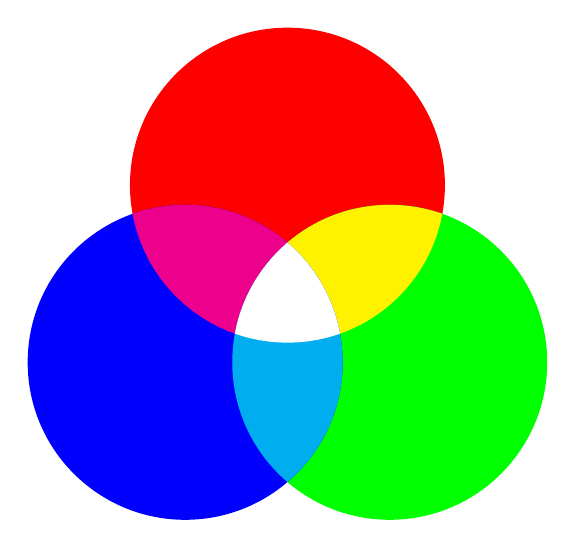
\begin{tikzpicture}

  \draw [draw=none, fill=red] (90:1.5) circle (2cm);
  \draw [draw=none, fill=green] (-30:1.5) circle (2cm);
  \draw [draw=none, fill=blue] (210:1.5) circle (2cm);

  \begin{scope}
    \clip (90:1.5) circle(2cm);
    \draw [draw=none, fill=yellow] (-30:1.5) circle (2cm);
  \end{scope}

  \begin{scope}
    \clip (210:1.5) circle(2cm);
    \draw [draw=none, fill=magenta] (90:1.5) circle (2cm);
  \end{scope}

  \begin{scope}
    \clip (-30:1.5) circle(2cm);
    \draw [draw=none, fill=cyan] (210:1.5) circle (2cm);
  \end{scope}

  \begin{scope} % red + green + blue = white
    \clip (90:1.5) circle(2cm);
    \clip (210:1.5) circle(2cm);
    \draw [draw=none, fill=white] (-30:1.5) circle (2cm);
  \end{scope}
\end{tikzpicture}
  \caption{RGB color model}
  \label{fig:rgb}
\end{figure}

The RGB color model relies on the fact that all colors are a mixture
of red,blue and green, as it is demonstrated in figure
\ref{fig:rgb}. White is a mixture of red, blue and green, yellow is
mixture of red and green, and so on. The mixing and matching of colors
can also be specified in numbers very easily, and that is something a
computer can very easily handle.

\section{Digtal image}
\label{sec:digtal-image}

% Images can most easily be thought of as an

\printbibliography[heading=subbibliography]
